\documentclass[]{article}
\usepackage{graphicx}
\usepackage{blindtext}
\usepackage{hyperref}
\graphicspath{ {./images/} }
\usepackage[spanish]{babel}
%opening
\title{Resumen sobre estadística y probabilidad.}
\author{Leandro Molina, Martin Borgo}

\hypersetup{
	colorlinks=true,
	linkcolor=blue,
	filecolor=magenta,      
	urlcolor=cyan,
	pdftitle={Overleaf Example},
	pdfpagemode=FullScreen,
}

\begin{document}

\maketitle
\vspace{-20pt}

\noindent

\includegraphics[width=\linewidth, height=14cm]{imagenes/twin_estadistica.png}
\footnote{Personaje perteneciente a \href{https://www.youtube.com/@TwinSensei}{Twin-Sensei}}
\pagebreak

\tableofcontents


\pagebreak
\section{Capitulo 1. ¿Que es la estadística?}
\subsection{¿Por qué se debe estudiar estadística?}
Hay 3 motivos para el estudio de la estadística estos son:
\begin{enumerate}
	\item La primera razón consiste en que la información numérica prolifera por todas partes. si revisas diarios o revistas contienen mucha cantidad de información numérica.
	\item Una segunda razón, es que las técnicas de la estadística se emplean para tomar decisiones que afectan la vida diaria, es decir, que incluyen en su bienestar.
	\item Una tercera razón, el conocimiento de sus métodos facilita la compresión de la forma en que se toman las decisiones y proporciona un entendimiento mas claro de como le afectan. 
\end{enumerate}
Al encarar la necesidad de tomar decisiones en las que tenes que saber hacer un análisis de datos resultara de utilidad. Con el fin de tomar una decisión informada, sera necesario llevar a cabo lo siguiente para poder tomar una decisión informada:
\begin{enumerate}
	\item Determinar si existe información adecuada o si requiere información adicional.
	\item Reunir información adicional, si se necesita, de manera que no se obtengan resultados erróneos.
	\item Resumir los datos de manera útil e informativa.
	\item Analizar la información disponible.
	\item Obtener conclusiones y hacer inferencias al mismo tiempo que se evaluá el riesgo de tomar una decisión incorrecta.
\end{enumerate}
En resumen hay por lo menos tres razones para estudiar estadística: 1) los datos proliferan por todas partes; 2) las técnicas estadísticas se emplean en la toma de decisiones que influyen en su vida; 3) sin que importe la carrera que elija, tomara decisiones profesionales que incluyan datos.

\subsection{¿Que se entiende por estadística?}
Posee dos significados: su aceptación más común, la estadística se refiere a información numérica. Una colección de información numérica recibe el nombre de \textbf{estadísticas}. La información estadística se presenta en forma gráfica, es útil porque capta la atención del lector e incluye una gran cantidad de información. 
\begin{flushleft}
\textbf{Estadística:} Ciencia que recoge, organiza, presenta, analiza e interpreta datos con el fin de propiciar una toma de decisiones mas eficaz.
\end{flushleft}
El primer paso en el estudio de un problema consiste en recoger datos relevantes. Estos deben organizarse de alguna forma y, tal vez, representarse en una gráfica.
\subsection{Tipos de estadística.}
El estudio de la estadística se divide en dos categorías: la estadística descriptiva y la estadística inferencial.
\subsubsection*{Estadística descriptiva.}
Es la ciencia que "recoge, organiza, presenta, analiza...datos". Esta parte de la estadística recibe el nombre de \textbf{estadística descriptiva}.

\begin{flushleft}
\textbf{Estadística descriptiva:} Métodos para organizar, resumir y presentar datos de manera informativa.
\end{flushleft}
Se trata de estadística descriptiva si calcula el crecimiento porcentual de una década a otra. Sin embargo, no seria de naturaleza descriptiva si utiliza estos para el calcular con esos datos algo futuro.
Una masa de datos desorganizados resulta de poca utilidad. Las técnicas de la estadística descriptiva permiten organizar esta clase de datos y darles significado. Los datos se ordenan en una \textbf{distribución de frecuencia} (mas adelante lo veremos). Se emplean diversas clases de \textbf{graficas} para describir datos.

\subsubsection*{Estadística inferencial.}
La estadística inferencial, también denominada \textbf{inferencia estadística}. El principal interés que despierta esta disciplina se relaciona con encontrar algo relacionado con una población a partir de una muestra de ella. Ya que estas son inferencias relacionadas con una población, basadas en datos de la muestra, se trata de estadística inferencial. Se podría considerar a la estadística inferencial como la mejor conjetura que es posible obtener del valor de una población sobre la base de la información de una muestra.
\begin{flushleft}
	\textbf{Estadística inferencial: }Métodos que se emplean para determinar una propiedad de una \textbf{población} con base en la información de una \textbf{muestra} de ella.
\end{flushleft}
Atención a las palabras población y muestra en la definición de estadística inferencial. Una \textbf{población} puede constar de individuos, también puede consistir en objetos. Desde una perspectiva estadística, una población no siempre que tiene que ver con personas.

\begin{flushleft}
	\textbf{Población: }Conjunto de individuos u objetos de interés o medidas que se obtienen a partir de todos los medios u objetos de interés.
\end{flushleft}
Con el objeto de inferir algo sobre una población, lo común es que se tome una muestra de ella.
\begin{flushleft}
	\textbf{Muestra: }Porción o parte de la población de interés.
\end{flushleft}
La toma de muestras para aprender algo sobre una población es de uso frecuente en administración, agricultura, política y acciones de gobierno.

\subsection{Tipos de variables.}
Una variable es una característica observable en las unidades estadísticas y tiene, por lo menos, dos valores. \\
Dos tipos básicos de variables: 1)Cualitativas y 2)Cuantitativas, la característica que se estudia es de naturaleza no numérica, recibe el nombre de \textbf{variable cualitativa} o \textbf{atributo}. Cuando los datos son de naturaleza cualitativa, importa la cantidad o proporción que caen dentro de cada categoría. Los datos cualitativos se resumen en tablas o graficas de barras. Cuando la variable que se estudia aparece en forma numérica, se le denomina \textbf{variable cuantitativa}. Las variables cuantitativas pueden ser discretas o continuas. Las \textbf{variables discretas} adoptan solo ciertos valores y existen vacíos entre ellos. Las variables discretas son el resultados de una relación numérica, las observaciones de una \textbf{variable continua} toman cualquier valor dentro de un intervalo especifico. Por lo general las variables continuas son el resultado de mediciones. \linebreak Resumen de los tipos de variables: \\
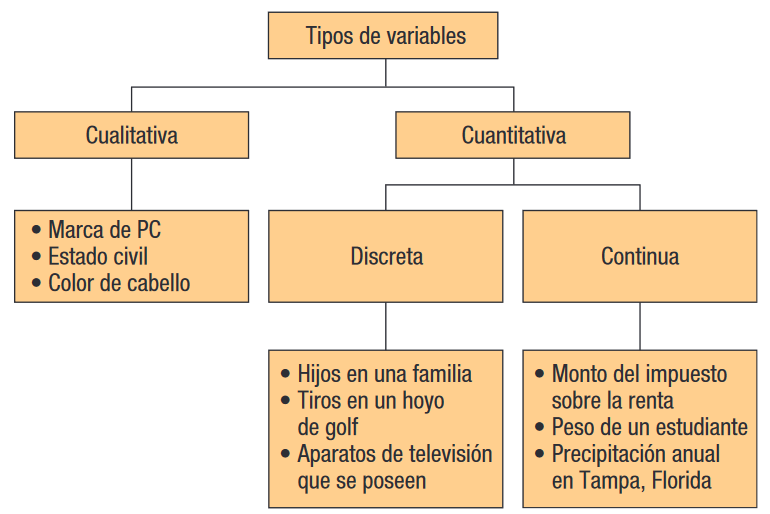
\includegraphics[width=14cm, height=8cm]{imagenes/resumenTiposVariables1_2}

\subsection{Niveles de medición.}
Los datos se clasifican por niveles de medición. El nivel de medición de los datos rige los cálculos que se llevan a cabo con el fin de resumir y presentar los datos. También determina las pruebas estadísticas que se deben realizar. De hecho, existen cuatro niveles de medición: nominal, ordinal, de intervalo y de razón. La medición mas baja, o mas primaria, corresponde al nivel nominal. La mas alta, o el nivel que proporciona la mayor información relacionada con la observación, es la medición de razón.

\subsubsection*{Datos de nivel nominal.}
Las observaciones acerca de una variable cualitativa solo se clasifican y se cuentan. No existe una forma particular para ordenar las etiquetas, no existe un orden natural. Para el nivel nominal, la medición consiste en contar, a veces, para una mejor compresión de lectura, estos conteos se convierten en porcentajes. Es necesario hacer que el porcentaje sume un total de 100\%, no existe un orden natural para los resultados. Para procesar datos a menudo se codifica la información en forma numérica. El nivel nominal tiene las siguientes propiedades:
\begin{enumerate}
	\item La variable de interés se divide en categorías o resultados.
	\item No existe un orden natural de los resultados.
	\item Los datos solo se clasifican.
\end{enumerate}

\subsubsection*{Datos de nivel ordinal.}
El nivel inmediato superior de datos es el \textbf{nivel ordinal}. No es posible distinguir la magnitud de las diferencias entre los grupos, ¿la diferencia entre superior y bueno es la misma que entre lo malo e inferior? No es posible afirmarlo. Las propiedades del nivel ordinal de los datos son las siguientes:
\begin{enumerate}
	\item Las clasificaciones de los datos se encuentran representadas por conjuntos de etiquetas o nombre (alto, medio, bajo), las cuales tienen valores relativos.
	\item En consecuencia, los valores relativos de los datos se pueden clasificar u ordenar.
\end{enumerate}

\subsubsection*{Datos de nivel de intervalo.}
\textbf{El nivel de intervalo} de medición es el nivel inmediato superior. Incluye todas las características de nivel ordinar, pero, ademas, la diferencia entre valores constituye una magnitud constante. Si las distancias entre los números tienen sentido, aunque las razones no, entonces tiene una escala de intervalo de medición. Las propiedades de los datos de nivel intervalo son las siguientes:
\begin{enumerate}
	\item Las clasificaciones de datos se ordenan de acuerdo con el grado que posea de las característica en cuestión.
	\item Diferencias iguales en la característica representan diferencias iguales en las mediciones (es decir la diferencia entre valores es significativa).
	\item El cero es relativo (no indica ausencia de estado).
\end{enumerate}

\subsubsection*{Datos de nivel de razón.}
Todos los datos cuantitativos son registrados en el nivel de razón de la medición, el \textbf{nivel de razón} es el \textit{mas alto}. Posee todas las características del nivel de intervalo, aunque, ademas, el punto 0 tiene sentido y la razón entre dos números significativa, si se encuentra en 0 significa la ausencia de algo (peso, dinero, etc). Las propiedades de los datos de nivel intervalo son las siguientes:
\begin{enumerate}
	\item Las clasificaciones de datos se ordenan de acuerdo con la cantidad de características que poseen.
	\item Diferencias iguales en la característica representan diferencias iguales en los números asignados a las clasificaciones.
	\item El punto cero representa la ausencia de características y la razón entre dos números es significativa.
	\item La razón entre valores es significativa.
\end{enumerate}
La siguiente grafica resume las principales características de los diversos niveles de medición.
\\
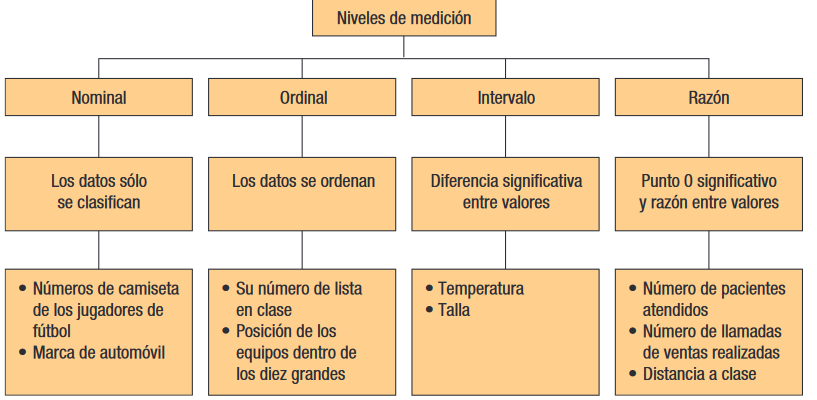
\includegraphics[width=16cm, height=8cm]{imagenes/resumenCaracteristicasNivelesMedicion1_3}
\section{Capitulo 2. Descripción de datos: tablas de frecuencias, distribuciones de frecuencias y su representación grafica.}
\subsection{Construcción de una tabla de frecuencias.}
La estadística descriptiva se encarga de organizar datos con el fin de mostrar la distribución general de estos y el lugar en donde tienden concentrarse, ademas de señalar valores de datos pocos usuales o extremos. El primer procedimiento que se emplea para organizar y resumir un conjunto de datos es una \textbf{tabla de frecuencias.}
\begin{center}
\textbf{Tabla de frecuencias:} Agrupación de datos cualitativos en clases mutuamente excluyentes que muestra el numero de observaciones en cada clase.
\end{center}
Recordar que, una variable cualitativa es de naturaleza no numérica; es decir, que la información es clasificable en distintas categorías. No hay un orden particular en estas categorías. Por otro lado, están las variables cuantitativas son de índole numérica.
\subsubsection*{Frecuencias relativas de clase.}
Es posible convertir las frecuencias de clase en frecuencias relativas de clase para mostrar la fracción del numero total de observaciones en cada una de ellas. Una frecuencia relativa capta la relación entre la totalidad de elementos de una clase y el numero total de observaciones. Para convertir una distribución de frecuencias en una distribución de frecuencias relativa, cada una de las frecuencias de clase se divide entre el total de observaciones.

\subsubsection*{Representación grafica de datos cualitativos.}
El instrumento mas común para representar una variable cualitativa en forma grafica es la \textbf{grafica de barras}. En la mayoría de los casos, el eje horizontal muestra la variable de interés y el eje vertical la frecuencia o fracción de cada uno de los posibles resultados. Una característica distinta de esta herramienta es que existe una distancia o espacio entre las barras. Una grafica de barras es una representación grafica de una tabla de frecuencias mediante una serie de rectángulos de anchura uniforme, cuya altura corresponde a la frecuencia de clase.
\begin{center}
\textbf{Grafica de barras:} En ella, las clases se representan en el eje horizontal y la frecuencia de clase en el eje vertical. Las frecuencias de clase son proporcionales a las alturas de las barras.
\end{center}
Se muestra ejemplo de una grafica de barras en la siguiente pagina:\\
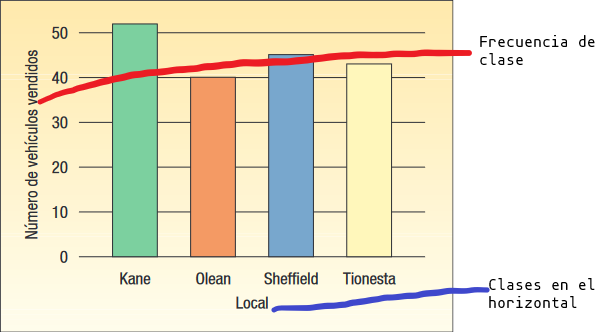
\includegraphics[width=13cm]{imagenes/graficaBarras2_1.png} \\
Otro tipo de grafica útil para describir información cualitativa es la \textbf{grafica de pastel}.
\begin{center}
	\textbf{Grafica de pastel: }Grafica que muestra la parte o porcentaje que representa cada clase del total de números de frecuencia.
\end{center}
El primer paso para elaborar una grafica de pastel consiste en registrar los porcentajes 0, 5, 10, 15, etc, de manera uniforme alrededor de la circunferencia de un circulo. El área rebanada representa alguna clase, cada rebanada de pastel representa la  porción relativa de cada componente, es posible compararlas con facilidad.\\
Acá un ejemplo de grafica bizcochuelo.\\
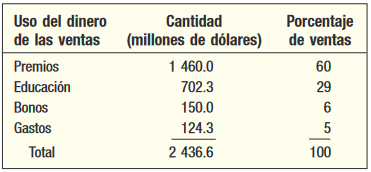
\includegraphics{imagenes/tablaFrecuenciasRelativas2_2.PNG}\\
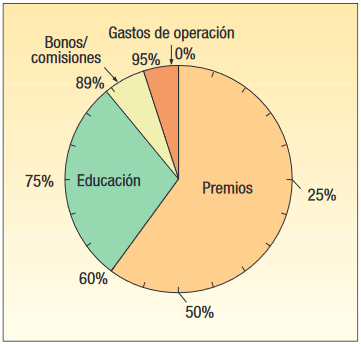
\includegraphics[width=12cm, height=10cm]{imagenes/graficoPastel2_2.png} \\
Las graficas de pastel y las de barras cumplen casi la misma función. ¿Cuales son los criterios para elegir una u otra? En la mayoría de los casos, las graficas de pastel son las mas informativas cuando se trata de comparar la diferencia relativa en el porcentaje de observaciones de cada uno de las variables de la escala nominal. Es preferible usar una grafica de barras cuando el objetivo es comparar el numero de observaciones en cada categoría.
\subsection{Construcción de distribuciones de frecuencias: datos cuantitativos.}
Distribución de frecuencias puede ser útil para describir la ganancias de ventas.
\begin{center}
	\textbf{Distribución de frecuencias: }Agrupación de datos en clases mutuamente excluyentes, que muestra el numero de observaciones que hay en cada clase.
\end{center}
¿Como crear una distribución de frecuencias? El primer paso consiste en acomodar los datos en una tabla que muestre las clases y el numero de observaciones que hay en cada clase. Recordá que el \textbf{objetivo} es construir tablas, diagramas y graficas que revelen rápidamente la concentración, los valores extremos y la distribución de los datos.
La información desorganizada como \textbf{datos en bruto} o \textbf{datos no agrupados}. Los datos en bruto se interpretan con mayor facilidad si se organizan como una distribución de frecuencias.\\
\textbf{Paso 1: Defina el numero de clases.} El objetivo consiste en emplear suficientes agrupamientos o \textbf{clases}, de manera tal que se perciba la forma de la distribución. Acá se necesita criterio. Una gran cantidad de clases o muy pocas podrían no permitir ver la conformación fundamental del conjunto datos. Una receta útil para determinar la cantidad de clases $(k)$ es la regla de 2 a la $k$. Esta guiá sugiere que se elija el menor numero $ (k) $ para el numero clases, de tal manera que $ 2^{k} $ sea mayor que el numero de observaciones $ (n) $. Ejemplo $ n=180 $ observaciones, si supone $ k=7 $, lo cual significa que utilizara siete clases, entonces $ 2^{7}=128 $, algo menos que las 180 observaciones. De ahí que 7 no represente suficientes clases. Si $ k=8 $, entonces $ 2^{8}=256$, que es mayor 180. Por lo tanto, el numero de clases se recomienda es de 8. \\\\
\textbf{Paso 2: Determine el intervalo o ancho de clase.} El \textbf{intervalo} o \textbf{ancho de clase} debería ser el mismo para todas las clases. Todas las clases juntas deben cubrir por lo menos la distancia del valor mas bajo al mas alto de los datos. Expresado esto en una formula seria:
\[ i\geq \frac{H-L}{k} \]
Por lo general el tamaño de intervalo se redondea a una cifra conveniente, tal como un múltiplo de 10 a 100. En las distribuciones de frecuencia son preferibles los intervalos de clase iguales. Sin embargo, en ciertos casos se necesita que no lo sean para evitar una gran cantidad de clases vacías, o casi vaciás.\\\\

\textbf{Paso 3: Establezca los limites de cada clase.} Este paso es importante para que sea posible incluir cada observación en una sola categoría. Esto significa que debe evitar la superposición de limites de clase confusos. Por ejemplo, clases como \$1300 - \$1400 y \$1400 - \$1500 no deberían emplearse porque no resulta claro si el valor de \$1400 pertenece a la primera o a la segunda clases. Las clases como \$1300 - \$1400 y \$1500 - \$1600 se emplean con frecuencia, aunque también pueden resultar confusas si no se conviene en redondear todos los datos de \$1450 o por arriba de esta cantidad a la segunda clase y los datos por debajo de \$1400 a la primera clase. Al redondear el intervalo de clase hacia arriba con el fin de obtener un tamaño conveniente de clase, se cubre un rango mas amplio que el necesario. Una directriz consiste en convertir el limite inferir de la primera clase en un múltiplo del intervalo de clase. A veces esto no es posible, pero el limite inferior por lo menos debe redondearse.\\\\
\textbf{Paso 4: Anote las veces que encuentre las observaciones en el intervalo en las clases.}  \textbf{PONER IMAGEN PASO 4}
\\\\\textbf{Paso 5: Cuente el numero de elementos de cada clase.}  El numero de elementos que hay en cada clase recibe el nombre de \textbf{frecuencia de clase.} Por ejemplo en numero de \$200 a \$600 hay 8 observaciones, y en la clase de \$600 a \$1000 hay 11 observaciones. Por lo tanto la frecuencia de clase de la primera es de 8, mientras que en la segunda es de 11. Hay un total de 180 observaciones o frecuencias en todo el conjunto de datos. así que la suma de todas las frecuencias debe ser igual a 180. \textbf{PONER TABLA2-7}\\\\
Con frecuencia aparecerán otros dos términos: \textbf{punto medio de clase} e \textbf{intervalo de clase.} El punto medio, que se encuentra entre los limites inferiores de dos clases consecutivas, se calcula sumando los limites interiores de clases consecutivas y dividiendo el resultado entre dos. En caso de la imagen del paso 5, el limite de clase interior de la primera clase es de \$200 y el siguiente limite es de \$600. El punto medio de clase \$400, que se calcula mediante la operación \[ \frac{\$600+\$200}{2} .\] El punto medio de \$400 representa mejor. Para determinar el intervalo de clase, se resta el limite inferior de la clase del limite inferior de la siguiente clase, es decir \[ \$600 -\$200 =400.\]Cambien se puede determinar el intervalo de clase calculando la diferencia entre puntos medios consecutivos. El punto medio de la primera clase des de \$400 y el punto medio de la segunda clase es de \$800. La diferencia es de \$400.
\subsection{Distribución de frecuencias relativas}
Si se requiere resumir las ventas del ultimo mes utilizando ganancia por venta; seria útil describir la ganancia de venta por medio de una distribución de frecuencias.
\begin{center}
	\textbf{Distribución de frecuencias: }Agrupación de datos en clases mutuamente excluyentes, que muestra el numero de observaciones que hay en cada clase.
\end{center}
¿Como crear una distribución de frecuencias? El primer paso consiste en acomodar los datos en una tabla que muestre las clases y el numero de observaciones que hay en cada clase. El objetivo es construir tablas, diagramas y graficas que revelen rápidamente la concentración, los valores extremos y la distribución de los datos. La información desorganizada como \textbf{datos en bruto} o \textbf{datos no agrupados.} Los datos en bruto se interpretan con mayor facilidad si se organizan como una distribución de frecuencias.\\\\
\textbf{Paso 1: Defina el numero de clases: }El objetivo consiste en emplear suficientes agrupamientos o \textbf{clases}, de manera tal que se perciba la forma de la distribución. Se necesita criterio. Una gran cantidad de clases o muy pocas podrían no permitir ver la conformación fundamental del conjunto de datos. Una receta útil para determinar la cantidad de clases (k) es la regla de 2 a la k. Esta guía sugiere que se elija el menor numero (k) para el numero de clases, de tal manera que \[2^{k}\] sea mayor que el numero de observaciones (n). Si $ n=180 $, si supone que $ k=7 $, lo cual significa que utilizara siete clases, entonces \[ 2^{7}=128 \], algo menos de 180. De ahí que 7 no represente suficiente clases. Si $ k=8 $, entonces \[ 2^{8}=256 \], que es mayor a 180. Por lo tanto, el numero de clases que se recomienda es de 8.\\\\
\textbf{Paso 2: Determine el intervalo o ancho de clase:} El \textbf{intervalo o ancho de clase} debería ser el mismo para todas las clases. Todas las clases juntas deben cubrir por lo menos la distancia del valor mas bajo al mas alto de los datos. Expresado esto en una formula seria: \[ i\geq\frac{H-L}{k} \] en la que la $ i $ es el intervalo de clase; H, el máximo valor observado; L, el mínimo valor observado, y k, el numero de clases. En la practica, por lo general este tamaño de intervalo se redondea a una cifra conveniente, tal como un múltiplo de 10 a 100. Las distribuciones de frecuencia son preferibles los intervalos de clase iguales. Ciertos casos se necesita que no lo sean para evitar una gran cantidad de clases vacías, o casi vacías. Facilita la compresión de la información.\\\\
\textbf{Paso 3: Establezca los limites de cada clase:} Este paso es importante para que esa posible incluir cada observación en una sola categoría. Esto significa que debe evitar la superposición de limites de clase confusos. Ponele tenes una clase 200-400 y otra de 400-600 ¿el 400 va incluido en la primera clase o en la segunda clase? ACLARA ESO O NO ENTIENDO NADADORA.\\\\
\textbf{Paso 4: Anote las observaciones en las clases:} Se da un ejemplo en la imagen siguiente \textbf{AGREGAR TABLA DEL PASO 4}\\\\
\textbf{Paso 5: Cuente el numero de elementos de cada clase:} El numero de elementos que hay en cada clase recibe el nombre \textbf{frecuencia de clase.} En la clase \$200 a \$600 hay 8 observaciones, y en la clase de \$600 a \$1000 hay 11 observaciones. Por lo tanto, la frecuencia de clase de la primera clase es de 8, mientras que en la segunda es de 11. Hay un total de 180 observaciones o frecuencias en todo el conjunto de datos. Así que la suma de todas las frecuencias debe ser igual a 180. \textbf{PEGAR TABLA2-7}
Las ventajas de condesar los datos de forma mas entendible y organizada compensa por mucho este desventaja. \linebreak[2]
Con frecuencia aparecerán otros dos términos: \textbf{punto medio de clase e intervalo de clase}. El punto medio, que se encuentra los limites inferiores de dos clases consecutivos, se calcula sumando los limites inferiores de clases consecutivas y dividiendo el resultado entre dos. Para determinar el intervalo de clase, se resta el limite inferior de la clase del limite inferior de la siguiente clase.
\subsection{Distribución de frecuencias relativas.}
Convertir frecuencias de clase en frecuencias relativas de clase, igual que con los datos cualitativos, con el fin de mostrar la fracción del total de observaciones que hay en cada clase. Una distribución de frecuencias relativas convierte la frecuencia en un porcentaje. Para convertir una distribución de frecuencia en una distribución de frecuencia relativa, cada una de las frecuencias de las clases se divide entre el numero total de observaciones. A continuación dejo la tabla de como serian una frecuencia relativa. \textbf{PONER TABLA 2-8}
\subsection{Representación grafica de una distribución de frecuencias.}
Es frecuente que se necesite una vista rápida de las tendencias de las ventas, los precios de las acciones o costos de hospitalización. A menudo, estas tendencias se describen por medio de tablas y graficas. Tres herramientas que serán de utilidad para representar gráficamente una distribución de frecuencias son el histograma, el polígono de frecuencias y el polígono de frecuencias acumuladas.
\subsubsection*{Histograma}
Un histograma de una distribución de frecuencias basadas en datos cuantitativos se asemeja mucho a la grafica de barras, que muestra la distribución de datos cualitativos. Las clases se señalan en el eje horizontal y las frecuencias de clase en el eje vertical. Las frecuencias de clase se representan por medio de las alturas de las barras. Existe una importante diferencia como consecuencia de la naturaleza de los datos. Por lo general, los datos cuantitativos se miden con escalas continuas, no discretas. Por lo tanto, el eje horizontal representa todos los valores posibles y las barras se colocan de forma adyacente para que muestren la naturaleza continua de los datos.
\begin{center}
	\textbf{Histograma: }Grafica en la que las clases se señalan en el eje horizontal y las frecuencias de clase en el eje vertical. Las frecuencias de clase se representan por medio de las altura de las barras, que se dibujan de manera adyacente.
\end{center}
Mostraremos un ejemplo a continuación.
\subsubsection*{Poligono de frecuencias}
Un polígono de frecuencias también muestra la forma que tiene una distribución y es similar a un histograma. Consiste en segmentos de recta que conectan los puntos que forman las intersecciones de los puntos medios de clase y frecuencias de clase. El punto medio de cada clase se indica en una escala en el eje X y las frecuencias de clase en el Y. Recordá que el punto medio de clase es el valor localizado en el centro de una clase y representa los valores típicos de ella (limite superior - limite inferior). La frecuencia de clase es el numero de observaciones que hay en una clase particular. Para construir un polígono de frecuencias, hay que desplazarse horizontalmente sobre la grafica al punto medio, y en seguida de manera vertical, la frecuencia de clase, donde se coloca un punto. Los valores X y de Y de este punto reciben el nombre de \textit{coordenadas}. El proceso continua con todas las clases. Posteriormente, los puntos se conectan de manera ordenada. Es decir, que el punto que representa la clase mas baja se une al que representa la segunda clase y así en lo sucesivo. \textbf{PONER GRAFICA 2-5}\linebreak Tanto el histograma como el polígono de frecuencias permiten tener una vista rápida de las principales características de los datos (máximos, mínimos, puntos de concentración, etc.). Aunque las dos representaciones tienen un propósito similar, el histograma posee la ventaja de que describe cada clase como un rectángulo, en el que la barra de altura de este representa el numero de elementos que hay en cada clase. El polígono de frecuencias, en cambio, tiene una ventaja con respecto al histograma. También permite comparar directamente dos o mas distribuciones de frecuencias \textbf{PONER GRAFICA 2-6 DE EJEMPLO}.
\subsubsection*{Distribuciones de frecuencia acumulativas}.
Una distribución de frecuencias acumulativas muestra el numero o porcentaje de observaciones por debajo de valores dados, con representación gráfica de un \textbf{polígono de frecuencias acumulativas.} Como su nombre lo indica, una distribución de frecuencias acumulativas y un polígono de frecuencias acumulativas implican \textit{frecuencias acumulativas}. La frecuencia acumulativa básicamente vas sumando todas las frecuencias de las clases. \textbf{PONER TABLA 2-9}
Para trazar una distribución de frecuencias acumulativas, \textbf{se ubica el limite superior de cada clase en una escala a lo largo del eje X}, y \textbf{las correspondientes frecuencias acumulativas, a lo largo del eje Y}. Para incluir información adicional, gradué el eje vertical a la izquierda en unidades y el eje vertical a la derecha en porcentajes.
\section{Capitulo 3. Descripción de datos: medidas numéricas.}
\subsection{Introducción}
En este capitulo se presentan dos formas numéricas de describir datos cuantitativos: las \textbf{medidas de ubicación} 
\footnote{La razón por la cual se llama \textit{medida de ubicación} es porque estas medidas estadísticas representan la posición o ubicación de los datos dentro de un conjunto de datos. Es decir, indican dónde se encuentra la mayoría de los valores de un conjunto de datos y cómo están distribuidos alrededor de esta posición central. Por ejemplo, la media aritmética es una medida de ubicación porque representa el valor central alrededor del cual se agrupan los demás valores en un conjunto de datos. La mediana, por otro lado, es una medida de ubicación porque representa el valor que divide el conjunto de datos en dos partes iguales, es decir, la mitad de los valores están por encima de la mediana y la otra mitad están por debajo.}
y las \textbf{medidas de dispersión.} A las medidas de ubicación a menudo se les llama \textbf{promedios}. El propósito de una medida de ubicación consiste en señalar el centro de un conjunto de valores. Vos ya estas conoces el concepto de promedio (media aritmética), medida de ubicación que muestra el valor central de los datos. Si solo tomas las medidas de ubicación en cuenta de un conjunto de datos o si compara varios conjuntos de datos utilizando valores centrales, llegara a una conclusión incorrecta. Ademas de las medidas de ubicación, debe tomar en consideración la \textbf{dispersión} (con frecuencia se le llama \textit{frecuencia variación }o \textit{propagación}) de los datos. Para describir la dispersión considere el rango, la desviación media, la varianza y la desviación estándar. En principio se explican las medidas de ubicación. No existe una única medida de dispersión; de hecho existen varias. Consideraremos cinco:
\begin{enumerate}
	\item La media aritmética.
	\item La media ponderada.
	\item La mediana.
	\item La moda.
	\item La media geométrica.
\end{enumerate}
La medida aritmética es la medida de ubicación que mas se utiliza y que se publica con mayor frecuencia, por lo cual se le considerará como parámetro para una población y como estadístico para las muestras.
\subsection{La media poblacional}
La media poblacional es la suma de todos los valores observados en la población dividida entre el numero de valores de la población. Para determinar la media poblacional, aplique la siguiente formula con la siguiente formula y formula con símbolos matemáticos:
\[ \mu=\frac{\sum X}{N} \] 
Cada símbolo representa:
\begin{itemize}
	\item $\mu$ representa la media poblacional; se trata de la letra minúscula griega mu.
	\item $N$ es la numera de valores en la población.
	\item $X$ representa cualquier valor particular.
	\item $\sum$ es la letra mayúscula griega sigma e indica la operación de suma.
	\item $\sum X$ es la suma de X valores en la población.
\end{itemize}
Cualquier característica medible de una población recibe el nombre de \textbf{parámetro}. La media de una población es un parámetro.
\begin{center}
	\textbf{Parámetro: }Característica de una población.
\end{center}

\subsection{Media de una muestra}
Con frecuencia se selecciona una muestra (Se menciono en el capitulo 1) de la población para estimar una característica especifica de la población. La \textit{media} es la suma de los valores de la muestra, divididos entre el numero total de valores de la muestra. La media de una muestra se determina de  la siguiente manera:
\[\overline{X} = \frac{\sum X}{n} \]
Cada símbolo representa:
\begin{itemize}
	\item $\overline{X}$ es la media de la muestra; se lee como "X barra."
	\item $n$ es el numero de valores de la muestra.
	\item $X$ representa cualquier valor particular.
	\item $\sum$ es la letra mayúscula griega sigma e indica la operación de suma.
	\item $\sum X$ es la suma de X valores en la población.
\end{itemize}
La media de una muestra o cualquier otra medición basada en una muestra de datos recibe el nombre de \textbf{estadístico}.
\begin{center}
	\textbf{Estadístico: }Característica de una muestra.
\end{center}

\subsection{Propiedades de la media aritmética}
La media aritmética es una medida de ubicación muy utilizada. Cuenta con algunas propiedades importantes:
\begin{enumerate}
	\item \textbf{Todo conjunto de datos de intervalo -o de nivel de razón- posee una media.} Recordá que en el capitulo 1 los datos de nivel de razón incluyen datos como edades, ingresos y pesos, y que la distancia entre los números es constante.
	\item \textbf{Todos los valores se encuentran incluidos en el calculo de la media.}
	\item \textbf{La media es única.} Solo existe una media en un conjunto de datos. Mas adelante en el capitulo que un promedio que podría aparecer dos o mas veces en un conjunto de datos.
	\item \textbf{La suma de las desviaciones de cada valor de la media es cero.} La media es un punto equilibrio de un conjunto de datos.
\end{enumerate}
La media tiene un punto débil. Recuerde que el valor de cada elemento de una muestra o población, se utiliza cuando se calcula la media. Si uno de estos valores son extremadamente grandes o pequeños comparadas con la mayoría de los datos, la media podría no ser un promedio adecuado para representar los datos. Es decir, la media se ve afectada en exceso por valores inusualmente grandes o pequeños.

\subsection{Media ponderada}
La media ponderada, que constituye un caso especial de la media aritmética, se presenta cuando hay varias observaciones con el mismo valor. Es una medida estadística que se utiliza para calcular el valor medio de un conjunto de datos, donde cada valor tiene un peso o una importancia específica. En la media ponderada, cada valor se multiplica por su peso y luego se divide por la suma de todos los pesos.
\[\overline{X_{w}} = \frac{\sum (wX)}{\sum w} \]
Observe que el denominador de una medida ponderada siempre es la suma de las ponderaciones.

\subsection{Mediana}
Ya se dijo que si los datos contienen uno o dos valores muy grandes o muy pequeños, la media aritmética no resulta representativa. Es posible describir el centro de dichos datos a partir de una medida de ubicación denominada \textbf{mediana}.
\begin{center}
	\textbf{Mediana: }Punto medio de los valores una vez que se han ordenado de menor a mayor o de mayor a menor.
\end{center}
Ordenas los datos y agarras el(o los) valor (valores) del medio (literalmente). ¿Como se determina la mediana en el caso de un numero par de observaciones? se ordenan las observaciones. En seguida, con el fin de obtener un único valor por convención, calcule la media de las dos observaciones medias. Así, en el caso de un numero par de observaciones, la mediana quizá no sea uno de los valores dados. Ejemplo ponele que tenes dos observaciones medias 5 y 7, la media de esos dos es 6.
Las principales propiedades de la mediana son las siguientes:
\begin{itemize}
	\item \textbf{No influyen en ella valores extremadamente grandes o pequeños.} Por consiguiente, la mediana es una valiosa medida de ubicación cuando dichos valores se presentan.
	\item \textbf{Es calculable en el caso de datos de nivel ordinal o mas altos.} Recordá que en el capitulo 1 que los datos de nivel ordinal pueden ordenarse de menor a mayor
\end{itemize}
La mediana se determina para cualquier nivel de datos, excepto los nominales.

\subsection{Moda}
La moda es otra medida de ubicación (promedio).
\begin{center}
	\textbf{Moda:} Valor de la observación que aparece con mayor frecuencia.
\end{center}
La moda es de especial utilidad para resumir datos de nivel nominal. Es posible determinar la moda para todos los niveles de datos: nominal, ordinal, de intervalo y de razón. La moda también tiene la ventaja de que no influyen en ella valores extremadamente grandes o pequeños. No obstante, la moda tiene sus desventajas, por las cuales se le utiliza con menor frecuencias que a la media o mediana. En el caso de muchos conjuntos de datos no existe la moda porque ningún valor se presenta mas de una vez. Puede ocurrir que un agrupamiento de datos tenga dos modas se denomina bi-modal (tiene dos modas).

\subsection{Posiciones relativas de la media, la mediana y la moda.}
Se trata de una distribución simétrica que también tiene forma de campana. Esta distribución \textit{posee} la misma forma a cualquier lado del centro. Si el polígono estuviera doblado a la mitad, las dos mitades serian idénticas. En cualquier distribución simétrica, la moda, la mediana, y la media siempre son iguales. Hay distribuciones simétricas que no tienen forma de campana (En una distribución en forma de campana la media, la mediana y la moda son iguales). Si una distribución no es simétrica, o \textbf{sesgada}, (Una distribución sesgada no es simétrica.) la relación entre las tres medidas cambia. En una distribución con sesgo positivo la media aritmética es la mayor de las tres medidas. ¿Por que? Porque en ella influyen, mas que sobre la mediana o la moda, unos cuantos valores extremadamente altos. Por lo general, la mediana es la siguiente medida mas grande en una distribución de frecuencias con sesgo positivo. La moda es la menor de las tres medidas. Si la distribución tiene un sesgo muy pronunciado, la media no seria una mediana adecuada. La mediana y la moda serian mas representativas. \\
Por el contrario, si una distribución tiene un \textbf{sesgo negativo}, la media es la menor medida de las tres. Por supuesto, la media es sensible a la influencia de una cantidad extremadamente pequeña de observaciones. La mediana es mayor que la media aritmética y la moda es la mas grande de las tres medidas. De nuevo, si la distribución tiene un sesgo muy pronunciado, la media no se utilizaría para representar a los datos.

\subsection{¿Por que estudiar la dispersión?}
Una medida de ubicación, como la media o la mediana, solo describe el centro de los datos. Desde este punto de vista resulta valiosa, pero no dice nada sobre la dispersión de los datos. Una medida de dispersión pequeña indica que los datos se acumulan con proximidad alrededor de la media aritmética. Por consiguiente, la media se considera representativa de los datos. Por el contrario, una medida grande de dispersión indica que la media no es confiable. Otra razón para estudiar la dispersión en un conjunto de datos consiste en comparar la propagación en dos o mas distribuciones. Una medida de dispersión sirve para evaluar la confiabilidad de dos o mas medidas de ubicación.

\subsection{Medidas de dispersión}
Consideraremos diversas medidas de dispersión. El rango se sustenta en los valores máximo y mínimo del conjunto de datos, es decir, solo se consideran dos valores. La desviación media, la varianza y la desviación estándar se basan en desviaciones de la media aritmética.

\subsection*{Rango}
La medida mas simple de dispersión es el \textbf{rango}. Representa la diferencia entre los valores máximo y mínimo de un conjunto de datos. En forma de ecuación:
\begin{quote}
	\item Rango = Valor máximo - valor mínimo
\end{quote}
El rango se emplea mucho en aplicaciones de control de procesos estadísticos (CPE), debido a que resulta fácil de calcular y entender.
\subsection{Rango intercuartílico o rango intercuartil}
El rango intercuartílico o rango intercuartil (RIC o IQR), se obtiene como la diferencia entre los cuartiles superior e inferior: RIC = \textbf{$Q_{3} - Q_{1}$} mide el rango del 50\% central de la distribución. Gráficamente, está asociado a la “caja” del diagrama de caja.
\subsection*{Desviación media}
Un problema que presenta el rango escriba en que parte de dos valores, el mas alto y el mas bajo, es decir, no los toma en cuenta a todos. La desviación media si lo hace; mide la cantidad media respecto de la cual los valores de una población o muestran varían. Expresado en forma de definición:
\begin{quotation}
	\item \textbf{Desviación media}: Media aritmética de los valores absolutos de las desviaciones con respecto a la media aritmética.
\end{quotation}
En el caso de una muestra, la desviación media, designada DM, se calcula mediante la formula:
\[  DM = \frac{\sum |X - \overline{X}\ |}{n}\]
en donde:
\begin{itemize}
	\item $X$ es el valor de cada observación.
	\item $\overline{X}$ es la media aritmética de los valores.
	\item $n$ es el numero de observaciones en la muestra.
	\item $||$ indica el valor absoluto.
\end{itemize}
¿Por que ignorar los signos de las desviaciones de la media? De no hacerlo, las desviaciones positivas y negativas se compensarían con exactitud unas a otras y la desviación media siempre seria cero. Dicha medida (cero) resultaría un estadístico sin utilidad.\\
La desviación media posee dos ventajas, primero, incluye todos los valores de los cálculos. Recuerde que el rango solo incluye los valores máximo y mínimo. Segundo, es fácil de definir: es la cantidad promedio que los valores se desvían de la media. Sin embargo, su inconveniente es el empleo de valores absolutos. Por lo general, es difícil trabajar con valores absolutos, así que la desviación media no se emplea con tanta frecuencia como otras medidas de dispersión, como la desviación estándar.

\subsection*{Varianza y desviación estándar}
La \textbf{varianza} y la \textbf{desviación estándar} también se fundamentan en las desviaciones de la media. Sin embargo, en lugar de trabajar con el valor absoluto de las desviaciones, la varianza y la desviación estándar lo hacen con el cuadrado de las desviaciones.
\begin{quote}
	\item \textbf{Varianza}: Media aritmética de las desviaciones de la media elevadas al cuadrado.
\end{quote}
La varianza es no negativa y es cero solo si todas las observaciones son las mismas.
El principal problema de la varianza es que se mide el términos del cuadrado de las unidades originales de medición. Por ejemplo:\\ Si las mediciones están dadas en metros, entonces la varianza queda expresada en metros cuadrados. Tomando la raíz cuadrada de la varianza, obtenemos la desviación estándar, que regresa la medida de variabilidad a la unidades de medición originales
\begin{quote}
	\item \textbf{Desviación estándar}: Raíz cuadrada de la varianza.
\end{quote}
La \textbf{desviación estándar} de un conjunto de mediciones es igual a la raíz cuadrada de la varianza.\\
Desviación estándar poblacional: $\delta = \sqrt{\delta^{2}}$\\
Desviación estándar muestral: $s = \sqrt{s^{2}}$
\subsection{Interpretación y usos de la desviación estándar}
La desviación estándar normalmente se utiliza como medida para comparar la dispersión de dos o mas conjuntos de observaciones.

\subsection{Coeficiente de variación}
El coeficiente de variación (CV) nos informa acerca de la dispersión \underline{relativa} de un conjunto de datos o mediciones.\\
Caso mediciones muéstrales: $CV = \frac{S}{|\overline{x}|}$\\
Caso mediciones poblacionales: $CV = \frac{\delta}{|\overline{\mu}|}$ \\
Principales características del CV:
\begin{enumerate}
	\item El coeficiente de variación no posee unidades, es decir es adimensional.
	\item Para su interpretación se puede expresar como porcentaje, teniendo en cuenta que puede superar el 100\%.
	\item Se utiliza para comparar conjuntos de datos pertenecientes a poblaciones distintas.
	\item Cuanto más grande es el coeficiente de variación más dispersos están los datos respecto de la media, por lo que la media va perdiendo representatividad.
\end{enumerate}
\subsection*{Teorema de Chebyshev}
Ya se ha insistido en el hecho de que una desviación estándar pequeña de un conjunto de valores indica que estos se localizan cerca de la media. Por el contrario, una desviación grande revela que las observaciones se encuentran muy dispersas con respecto a la media. El pibe Chebyshev estableció un teorema que nos permite determinar la mínima porción de valores que se encuentran a cierta cantidad de desviaciones estándares de la media.  El teorema del Cheby establece lo siguiente:
\begin{quote}
	\item \textbf{Teorema de Chebyshev}: En cualquier conjunto de observaciones  (muestra o población), la proporción de valores que se encuentran a $k$ desviaciones estándares de la media es de por lo menos $1 - 1/k^{2}$, siendo $k$ cualquier constante mayor que 1.
\end{quote}

\subsection*{La regla empírica}
El teorema Cheby se relaciona con cualquier conjunto de valores; es decir, que la distribución de valores puede tener cierta forma. Sin embargo, en cualquier distribución simétrica con forma de campana, es posible ser mas precisos en la explicación de la dispersión en torno a la media. Estas relaciones que implican la desviación estándar y la media se encuentran descritas en la \textbf{regla empírica}, a veces denominada \textbf{regla normal}. La regla empírica solo se aplica a distribuciones simétricas con forma de campana.

\begin{quote}
	\textbf{Regla empírica}: En cualquier distribución de frecuencias simétrica con forma de campana, aproximadamente 68\% de las observaciones se encontraran entre mas y menos una desviación estándar de la media; cerca de 95\% de las observaciones se encontraran entre mas y menos dos desviaciones estándares de la media y, de hecho (99.7\%), estarán mas y metros tres desviaciones de la media.
\end{quote}
Se ha observado que si una distribución es simétrica y tiene forma de campana, todas las observaciones se encuentran entre la media y menos tres desviaciones estándares.

\subsection{Media y desviación estándar de datos agrupados}
En la mayoría de los casos las medidas de ubicación, como la media y las medidas de dispersión, como la desviación estándar, se determinan utilizando valores individuales. Sin embargo, algunas veces solo se cuenta con la distribución de frecuencias y se desea calcular la media o la desviación estándar. La siguiente explicación explica como calcular la media y la desviación estándar a partir de datos organizados en una distribución de frecuencias. Hay que insistir en que una media o una desviación estándar de datos agrupados es una estimación de los valores reales correspondientes.

\subsection*{Media aritmética}
Para aproximar la media aritmética de datos organizados en una distribución de frecuencia, comience suponiendo que las observaciones en cada clase se representan a través del punto medio de la clase. La media de una muestra de datos organizados en una distribución de frecuencias se calcula de la siguiente manera:

\begin{quote}
	\item \textbf{Media aritmética de datos agrupados}: \[ \overline{X} = \frac{\sum fM}{n} \]
	donde:
	\item $\overline{X}$ designa la media muestra.
	\item  $M$ es el punto medio de cada clase.
	\item $f$ es la frecuencia en cada clase.
	\item $fM$ es la frecuencia en cada clase multiplicada por el punto medio de la clase.
	\item $\sum fM$ es la suma de estos productos.
	\item $n$ es el numero total de frecuencias.
\end{quote}

\subsection*{Desviación estándar}
Para calcular la desviación estándar de datos agrupados en una distribución de frecuencias, necesita ajustar ligeramente la formula. Pondere cada una de las diferencias cuadradas por el numero de frecuencias en cada clase. La formula  de la \textbf{Desviación estándar, datos agrupados} es:
\[ s = \sqrt{\frac{\sum f(M - \overline{X})^{2}}{n - 1}}\]
donde:
\begin{quote}
	\item $s$ es el símbolo de la desviación estándar de la muestra.
	\item $M$ es el punto medio de la clase.
	\item $f$ es la frecuencia de clase.
	\item $n$ es el numero de observaciones en la muestra.
	\item $\overline{X}$ designa la media muestra.
\end{quote}

\subsection{Ética e informe de resultados}
Esta aprendiendo a organizar, resumir e interpretar datos mediante la estadística, también es importante que comprenda esta disciplina con el fin de que se convierta en un consumir inteligente de información. En este capitulo aprendió la forma de calcular estadísticas descriptivas de naturaleza numérica. En particular, la manera de calcular e interpretar medidas de ubicación de un conjunto de datos: la media, la mediana y la moda. También ha estudiado las ventajas y desventajas de cada estadístico. Conocer las ventajas y desventajas de la media, la mediana y la moda es importante al dar un informe estadístico y cuando se emplea información estadística para tomar decisiones. También aprendió a calcular medidas de dispersión: el rango, la desviación media y la desviación estándar. Cada uno de estos estadísticos tiene ventajas y desventajas. Recuerde que el rango proporciona información sobre la dispersión total de una distribución. Sin embargo, no aporta información sobre la forma en que se acumulan los datos o se concentran entorno al centro de la distribución. Conforme aprenda más estadística, necesitara recordar que  cuando emplea esta disciplina debe mantener un punto de vista independiente y basado en principios. Cualquier informe estadístico requiere la comunicación honesta y objetiva de los resultados.

\section{Descripción de datos}
En este capítulo continua el estudio de la estadística descriptiva. Estos diagramas y la estadística proporcionan una idea adicional del lugar en el que los valores se concentran, así como de la forma general de los datos. En seguida se consideran datos bivariados de cada una de las observaciones individuales o seleccionadas.
\begin{quote}
	\textbf{Parámetros}: medidas descriptivas numéricas calculadas a partir de \textbf{mediciones poblacionales.} Por ejemplo, la media aritmética o promedio de una población, es decir, la media poblacional.
	\item \textbf{Estadísticos (o estadísticas)}: medidas descriptivas numéricas calculadas a partir de \textbf{mediciones muéstrales.} Por ejemplo, la media aritmética o promedio de una muestra, es decir, la media muestral
\end{quote}
Los parámetros se designan con \textbf{letras griegas} y los estadísticos con \textbf{letras latinas}, a veces con algún añadido como el caso de la media (con una barra arriba de la letra).
\subsection{Sesgo}
Hay cuatro formas: simétrica, con sesgo positivo, con sesgo negativo y bimodal. En un conjunto \textbf{simétrico} de observaciones la media y mediana son iguales, y los valores de datos se dispersan uniformemente en torno a estos valores. Un conjunto de valores se encuentra \textbf{sesgado a la derecha} o \textbf{positivamente sesgado} o \textbf{sesgado a la izquierda} si existe un solo pico y los valores a se extienden mucho mas allá a la derecha del pico que a la izquierda de este. En este caso \textbf{la media es mas grande que la mediana}. En una distribución \textbf{negativamente sesgada} existe un solo pico, pero las observaciones se extienden mas a la izquierda, en dirección negativa. En una distribución negativamente sesgada, \textbf{la media es menor que la mediana}. Una \textbf{distribución bimodal} tendrá dos o mas picos. Con frecuencia este es el caso cuando los valores provienen de dos o mas poblaciones
\subsection{Percentiles, deciles y cuartiles}
La desviación estándar es la medida de dispersión que mas se utiliza. No obstante, existen otras formas de describir la variación o dispersión de un conjunto de datos. Un método consiste en determinar la ubicación de los valores que dividen un conjunto de observaciones en partes iguales. Estas medidas incluyen los \textbf{cuartiles, deciles y percentiles}.\\
Los \textbf{cuartiles} dividen a un conjunto de observaciones en cuatro partes iguales, ordenadas de menor a mayor. Para explicarlo mejor, piense en un conjunto de valores ordenados de menor a mayor. Anteriormente se denomino a la \textit{mediana} al valor intermedio de un conjunto de datos ordenados de menor a mayor. Es decir el 50\% de las observaciones son mayores que la mediana y 50\% son menores que la mediana. La mediana constituye una medida de ubicación, ya que señala el centro de los datos. De igual manera, los \textbf{cuartiles} dividen a un conjunto de observaciones en cuatro partes iguales. El primer cuartil, que se representa con $Q_{1}$, es el valor debajo del cual se presenta el 25\% de las observaciones, y el tercer cuartil, que simboliza $Q_{3}$, es el valor debajo del cual se presenta 75\% de las observaciones. Lógicamente, $Q_{2}$ es la mediana. $Q_{1}$ puede considerarse  como la mediana de la mitad inferior y $Q_{3}$ como la mediana de la parte superior de los datos. \\
Asimismo, los \textbf{deciles} dividen un conjunto de observaciones en 10 partes iguales y los \textbf{percentiles} en 100 partes iguales.\\Un ejemplo de deciles es, si su promedio general en la universidad se encuentra en el octavo decil, usted podría concluir que 80\% de los estudiantes tuvieron un promedio general inferior al suyo y 20\%, un promedio superior. \\ Un ejemplo de percentiles es, un promedio general ubicado en el trigésimo tercer percentil significa que el 33\% de los estudiantes tienen un promedio general mas bajo y que el 67\% un promedio mas alto.
\subsection{Diagramas de caja}
Un \textbf{diagrama de caja} o \textbf{box-plot} es una representación grafica, basada en cuartiles, que ayuda a presentar un conjunto de datos. Para construir un diagrama de caja, solo necesita cinco estadísticos:
\begin{enumerate}
	\item El valor mínimo.
	\item Primer cuartil.
	\item La mediana (segundo cuartil).
	\item Tercer cuartil.
	\item El valor máximo.
\end{enumerate}
\subsection*{Construcción de un diagrama de caja}
Cualquier medición a mayor distancia del límite superior o mayor distancia del límite inferior es un resultado o valor atípico; el resto de las mediciones, dentro de los límites, no son inusuales. Los resultados atípicos se suelen marcar con un asterisco o punto. El diagrama de caja marca el rango del conjunto de datos usando “bigotes” para conectar las mediciones más pequeñas y más grandes (excluyendo resultados atípicos) a la caja.
\begin{quote}
	\textbf{Límite inferior}: $Q_{1} - 1,5.(Q_{3} - Q_{1})$
	\item \textbf{Límite superior}: $Q_{3} + 1,5.(Q_{3} - Q_{1})$
\end{quote}
\textbf{Importante: }Los límites son imaginarios, no se suelen trazar
A la diferencia \textbf{$Q_{3} - Q_{1}$} se le llama \textbf{rango intercuartílico} o \textbf{rango intercuartil}.
Un diagrama de caja puede representarse de manera horizontal o vertical. Suele ser más sencillo de interpretar de manera horizontal.
\pagebreak
\section{Probabilidad}
A la estadística descriptiva le concierne el resumen de datos recogidos de eventos pasados. Ahora se presenta la segunda faceta de la estadística, a saber, el \textit{calculo de la probabilidad de que algo ocurra en el futuro}. Esta faceta de la estadística recibe el nombre de \textbf{inferencia estadística} o \textbf{estadística inferencial}. La inferencia estadística se relaciona con las conclusiones relacionadas con una población sobre la base de una muestra que se toma de ella. Dada la incertidumbre existente en la toma de decisiones, es importante que se evalúen científicamente todos los riesgos implicados. La teoría de la probabilidad, a menudo conocida como la ciencia de la incertidumbre, resulta útil para hacer esta evaluación. Su aplicación permite a quien toma decisiones y posee información limitada analizar los riesgos y reducir al mínimo el riesgo que existe, por ejemplo, al lanzar al mercado un nuevo producto o aceptar un envió que contenga partes defectuosas. Puesto que los conceptos de la probabilidad son importantes en el campo de la inferencia estadística, en este capitulo se introduce el lenguaje básico de la probabilidad, que incluye términos como experimento, evento, probabilidad subjetiva y reglas de la adición y de la multiplicación.
\subsection{¿Que es la probabilidad?}
En general es un numero que describe la posibilidad de que algo suceda.
\begin{quote}
	\textbf{Probabilidad}: Valor entre cero y uno, inclusive, que describe la posibilidad relativa (oportunidad o casualidad) de ocurra un evento.
\end{quote}
Es común que una probabilidad sea expresada en forma décima, como 0.70, 0.27 o 0.50. No obstante, también se da forma de fracción, como 7/10, 27/100 o 1/2. Se puede suponer cualquier numero de 0 a 1, inclusive. La probabilidad de 1 representa algo que seguramente sucederá, y la probabilidad de 0 representa algo que no sucederá. Cuanto mas próxima se encuentre una probabilidad a 0, mas improbable es que el evento suceda. Cuanto mas próxima se encuentre la probabilidad a 1, mas seguro que suceda. En el estudio de la probabilidad se utilizan tres palabras clave: \textbf{experimento, resultado} y \textbf{evento}.
\begin{quote}
	\textbf{Experimento}: Proceso que induce a que ocurra una y solo una de varias posibles observaciones.
\end{quote}
Respecto de la probabilidad, un experimento tiene dos o mas posibles resultados y no sabe cual ocurrirá.
\begin{quote}
	\textbf{Resultado}: Resultado particular de un experimento.
\end{quote}
Un ejemplo: lanzar una moneda al aire constituye un experimento. Usted puede observar el lanzamiento de una moneda, pero no esta seguro si caerá \textit{cara} o \textit{cruz}. Si se lanza una moneda, un resultado particular es \textit{cara}. El otro posible resultado es \textit{cruz}. Cuando se observan uno o mas resultados en los experimentos constituyen un evento.
\begin{quote}
	\textbf{Evento}: Conjunto de uno o mas resultados de un experimento.
\end{quote}
Un ejemplo: En el caso del experimento del lanzamiento de un dado, hay seis posibles resultados, pero existen varios posibles eventos. Cuando se cuenta el numero de miembros de la junta directiva de las compañías de Fortune 500 que tienen mas de 60 años de antigüedad el numero posibles de resultados varia de cero al total de miembros. Hay un numero aun mayor de eventos posibles en este experimento.
\textbf{PONER TABLA PAGINA 147, CAP 5.2 ¿que es la probabilidad?}
\subsection{Enfoques para asignar probabilidades.}
\subsubsection*{Probabilidad clásica.}
\subsubsection*{Probabilidad empírica.}
\subsubsection*{Probabilidad subjetiva.}

\subsection{Teorema de Bayes}
El teorema de Bayes es un caso de aplicación de la probabilidad condicional, el cual se puede aplicar cuando se cuenta con información a priori de los datos que se están analizando. Pero para comenzar a introducirnos a este teorema primero tenemos que tener en cuenta una serie de cosas.
\begin{enumerate}
	\item Tener conocimiento de que es un diagrama de árbol, como leerlos y como este nos va a ayudar en el planteamiento del problema.
	\item El concepto de probabilidad total de un evento.
	\item La regla general de la multiplicación, que se utiliza para obtener la fórmula del teorema de Bayes.
\end{enumerate}
\subsubsection*{Diagrama de Árbol}
Los diagramas de árbol, son una forma de representar las distintas condiciones o alternativas a las que están sometidas las variables de un problema, para su mejor comprensión supongamos que nos encontramos con el siguiente problema:
El 0,1\% de la población de un país está infectada con una bacteria, y la prueba para detectar la enfermedad tiene una efectividad del 99\% en las personas enfermas y para las personas que no están infectadas este porcentaje es de 2\%.
Con fin de representar estos datos de forma más gráfica y ordenada, podemos poner toda esta información en un diagrama de árbol, el cual quedaría conformado de la siguiente manera.

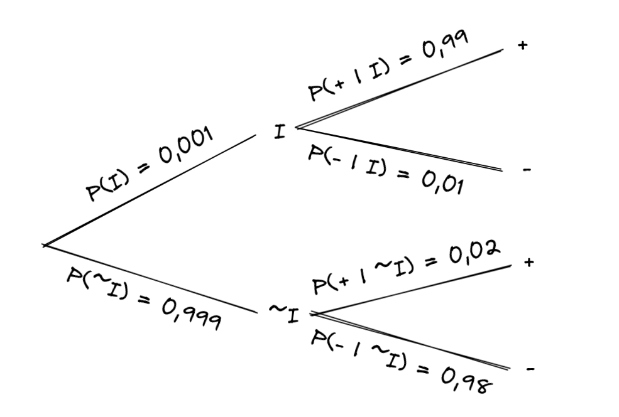
\includegraphics[width=12cm, height=10cm]{imagenes/diagrama_arbol.png}
Como se puede observar cada rama del árbol contiene los respectivos valores representativos para cada situación. Un dato importante a tener en cuenta a la hora de realizar este tipo de diagrama es que la suma de las probabilidades de las ramas pertenecientes al mismo padre deben dar siempre 1, por ejemplo, si la probabilidad de estar infectado es de 0,001 entonces la de no estar infectado debe ser si o si 0,999; ya que la sumas de estos dos siempre tiene que dar 1.
\subsubsection*{Teorema de la Probabilidad Total}
Siguiendo con el ejemplo presentado anteriormente, supongamos que queremos saber cual es la probabilidad de que una persona de positiva en la prueba, independientemente de si está infectado con la bacteria o no.
En ese caso se tendrán que sumar todos los caminos posibles del diagrama de árbol que nos lleve hacia ese evento específico. Aunque ya existe una fórmula que nos facilita encontrar la probabilidad total.
\[ \sum_{j=1}^{k} P(S_j)P(A|S_j) \]
Nótese que en sí esta ecuación en primera instancia es la sumatoria de las intersecciones entre los demás eventos del experimento, con el evento que nosotros estamos analizando, en nuestro caso cuál es la probabilidad de que de positivo una prueba, independientemente de si está infectado o no. Dicha sumatoria nos quedaría de la siguiente manera.
\[ \sum_{j=1}^{k} S_j \cap A \]
Esta fórmula se transforma, en la del teorema de la probabilidad total, si aplicamos la regla general de la multiplicación, en la cual una intersección entre eventos se puede representar como la multiplicación de la siguiente manera:
\begin{quote}
	\item $P(S \cap A) = P(S)P(A|S)$
	\item $P(S \cap A) = P(A)P(S|A)$
\end{quote}
\subsubsection*{Fórmula del Teorema de Bayes}
Supongamos ahora que queremos saber la probabilidad de que la prueba de positiva siendo que estas infectado con la bacteria. En ese caso ese valor sería obtenido a través de la siguiente fórmula:
\[ P(S_i|A)= \frac{P(S_i)P(A|S_i)}{\sum_{j=1}^k P(S_j)P(A|S_j)} \]
Como podemos ver, esta fórmula es la misma que para la probabilidad condicionada, con la diferencia que se realiza una serie de cambios leves, resultado de aplicar las propiedades antes mencionadas.
Este teorema resulta muy útil para muchos campos de la ciencia. Pero tiene una serie de puntos débiles que lo convierten en una no muy buena opción para algunas situaciones en particular.
\begin{enumerate}
	\item Si no se tiene un conocimiento del fenómeno, no es posible asignar las probabilidades iniciales (a priori) y por lo tanto no es posible aplicar el teorema de Bayes. Este problema se suele evitar, suponiendo que las probabilidades a priori tienen una distribución uniforme, lo cual es considerado por algunos autores como inaceptable, porque en muchas situaciones no conocemos la distribución inicial, pero sabemos claramente que no es uniforme. Otra posibilidad sería asignar subjetivamente las probabilidades iniciales, es decir asignar probabilidad sin contar con evidencias que la respaldan, pero esto llevaría a que dos investigadores con los mismos datos obtuviesen unas probabilidades finales diferentes.
	\item El método de Bayes no permite calcular ni revisar "\textit{probabilidades a priori objetivas}" de la hipótesis sino las "\textit{probabilidades a priori subjetivas}" de dicha hipótesis, la cual es establecida por cada investigador. Es decir su grado personal de creencia en la veracidad de la hipótesis.
\end{enumerate}
\end{document}
